% Article type supporting font formatting
\documentclass[a4,12pt]{extarticle}

% Define .tex file encoding
\usepackage[utf8]{inputenc}

% Norwegian language support
%\usepackage[norsk]{babel}     

% Indent first paragraph in section
\usepackage{indentfirst}

% Allows mathbb in tex file
\usepackage{amsfonts}    
     
% Margin defining package
\usepackage{geometry}         
\geometry{a4paper
  ,margin=1in
}

\usepackage[square,numbers]{natbib}

% For use of graphics in document
\usepackage{graphicx}         

% Allows multi-line comments in tex file
\usepackage{verbatim}         

% Allows math in tex file 
\usepackage{amsmath}          

% Allows math symbols in tex file
\usepackage{amssymb}          

% Allows use of physics shortcut functions
%\usepackage{physics}          

% Verbatim env with LaTeX commands
\usepackage{alltt}            

% Allows \begin{figure}[H]
\usepackage{float}            

% Necessary for defining colours
\usepackage{color}            
\definecolor{linkgreen}{rgb}{0,.5,0}
\definecolor{linkblue}{rgb}{0,0,.5}
\definecolor{linkred}{rgb}{.5,0,0}
\definecolor{blue}{rgb}{.13,.13,1}
\definecolor{green}{rgb}{0,.5,0}
\definecolor{red}{rgb}{.9,0,0}

% Hyperlinks in document
\usepackage{hyperref}  
\hypersetup{
  colorlinks=true,     % True for colored links
  linktoc=all,         % True for table of contents links
  linkcolor=linkblue,  % Colour for links
  urlcolor=linkgreen,  % Colour for URLs
  citecolor=linkred    % Colour for citations
}

% Listing package for code examples
\usepackage{listings}         
\lstset{
  language=C++,                % Set language to C++
  showspaces=false,            % Don't show space chars
  showtabs=false,              % Don't show tab chars
  breaklines=true,             % Break long lines of code
  showstringspaces=false,      % Don't show spaces in strings
  breakatwhitespace=true,      % Break at white space only
  commentstyle=\color{green},  % Set colour for comments
  keywordstyle=\color{blue},   % Set colours for keywords
  stringstyle=\color{red},     % Set colour for strings
  basicstyle=\ttfamily,        % Set basic style
  tabsize=2                    % Set tabsize
}

% Referencing, last for compatibility reasons
\usepackage[noabbrev]{cleveref}

% Command to set two lines under text
\newcommand{\uunderline}[1]{\underline{\underline{#1}}}

% Command to use integral with limits
\newcommand{\Int}{\int\limits}    

% Command to use double integral with limits
\newcommand{\IInt}{\iint\limits}  

% Command to use triple integral with limits
\newcommand{\IIInt}{\iiint\limits}

% Command removes section numbering
\newcommand{\mysection}[2]{   
\setcounter{section}{#1}
\section*{#2}
\addcontentsline{toc}{section}{#2}
}

% Command removes subsection numbering
\newcommand{\mysubsection}[2]{  
\setcounter{subsection}{#1}
\subsection*{#2}
\addcontentsline{toc}{subsection}{#2}
}

% Command removes subsubsection numbering
\newcommand{\mysubsubsection}[2]{ 
\setcounter{subsubsection}{#1}
\subsubsection*{#2}
\addcontentsline{toc}{subsubsection}{#2}
}

% Makes matrices look square-ish
\renewcommand*{\arraystretch}{1.5}

%%%%%%%%%%%%%%%%%%%%%%%%%%%%%%%%%%%%%%%
%%      Title, Author, and Date      %%
%%%%%%%%%%%%%%%%%%%%%%%%%%%%%%%%%%%%%%%
\title{Assignment 2 in Artificial Intelligence\\Spring 2018 }
\author{Daniel Aaron Salwerowicz}
\date{\today}

%%%%%%%%%%%%%%%%%%%%%%%%%%%%%%%%%%%%%%%
%%           Start document          %%
%%%%%%%%%%%%%%%%%%%%%%%%%%%%%%%%%%%%%%%
\begin{document}
  
%%%%%%%%%%%%%%%%%%%%%%%%%%%%%%%%%%%%%%%
%%   Create the main title section   %%
%%%%%%%%%%%%%%%%%%%%%%%%%%%%%%%%%%%%%%%
\maketitle

%%%%%%%%%%%%%%%%%%%%%%%%%%%%%%%%%%%%%%%
%%      Abstract for the report      %%
%%%%%%%%%%%%%%%%%%%%%%%%%%%%%%%%%%%%%%%
%\begin{abstract} 
%Say why this report exists. Motivations behind it and what not.
%\end{abstract}

%%%%%%%%%%%%%%%%%%%%%%%%%%%%%%%%%%%%%%%
%%         ToC for the report        %%
%%%%%%%%%%%%%%%%%%%%%%%%%%%%%%%%%%%%%%%
%\tableofcontents
%\pagebreak

%%%%%%%%%%%%%%%%%%%%%%%%%%%%%%%%%%%%%%
%%  The main content of the report  %%
%%%%%%%%%%%%%%%%%%%%%%%%%%%%%%%%%%%%%%

\mysection{1}{Exercise 2}
  \mysubsection{1}{A}
  Turing test is meant to be a test for AI to see how "Human-like" it is. In simple case you have an interrogator who communicates with two entities whom he cannot see, hear or feel. He can only use responses to his questions to determine which one of the two entities is a human and which one is an AI.
  
  \mysubsection{2}{B}
  Entity that we would qualify as an agent is characterized by observing, evaluating and acting upon its environment in order to achieve its goals. There are human, software and robotic agents.
  \begin{figure}[H]
    \centering
    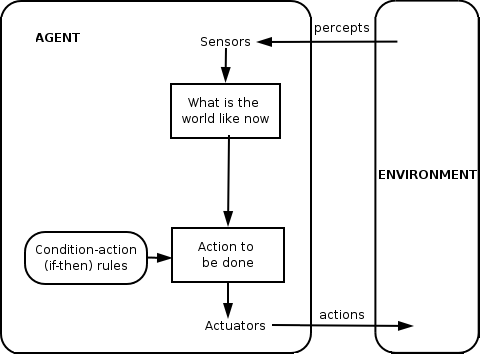
\includegraphics[width=.6\textwidth]{2b}
    \caption{Example drawing of an agent. Courtesy of Utkarshraj Atmaram via commons.wikimedia.org}
  \end{figure}
  
  \mysubsection{3}{C}
  As I understand it a state space is a representation of all states that a given system can have. For example all possible chess pieces configurations on chess board or all possible combinations of playing cards in a deck.
  
  As such a graph is a really great way of representing connections in such a system since it can show how these states are connected. In other words how you can get from one state of chess board to the other.
  \begin{figure}[H]
    \centering
    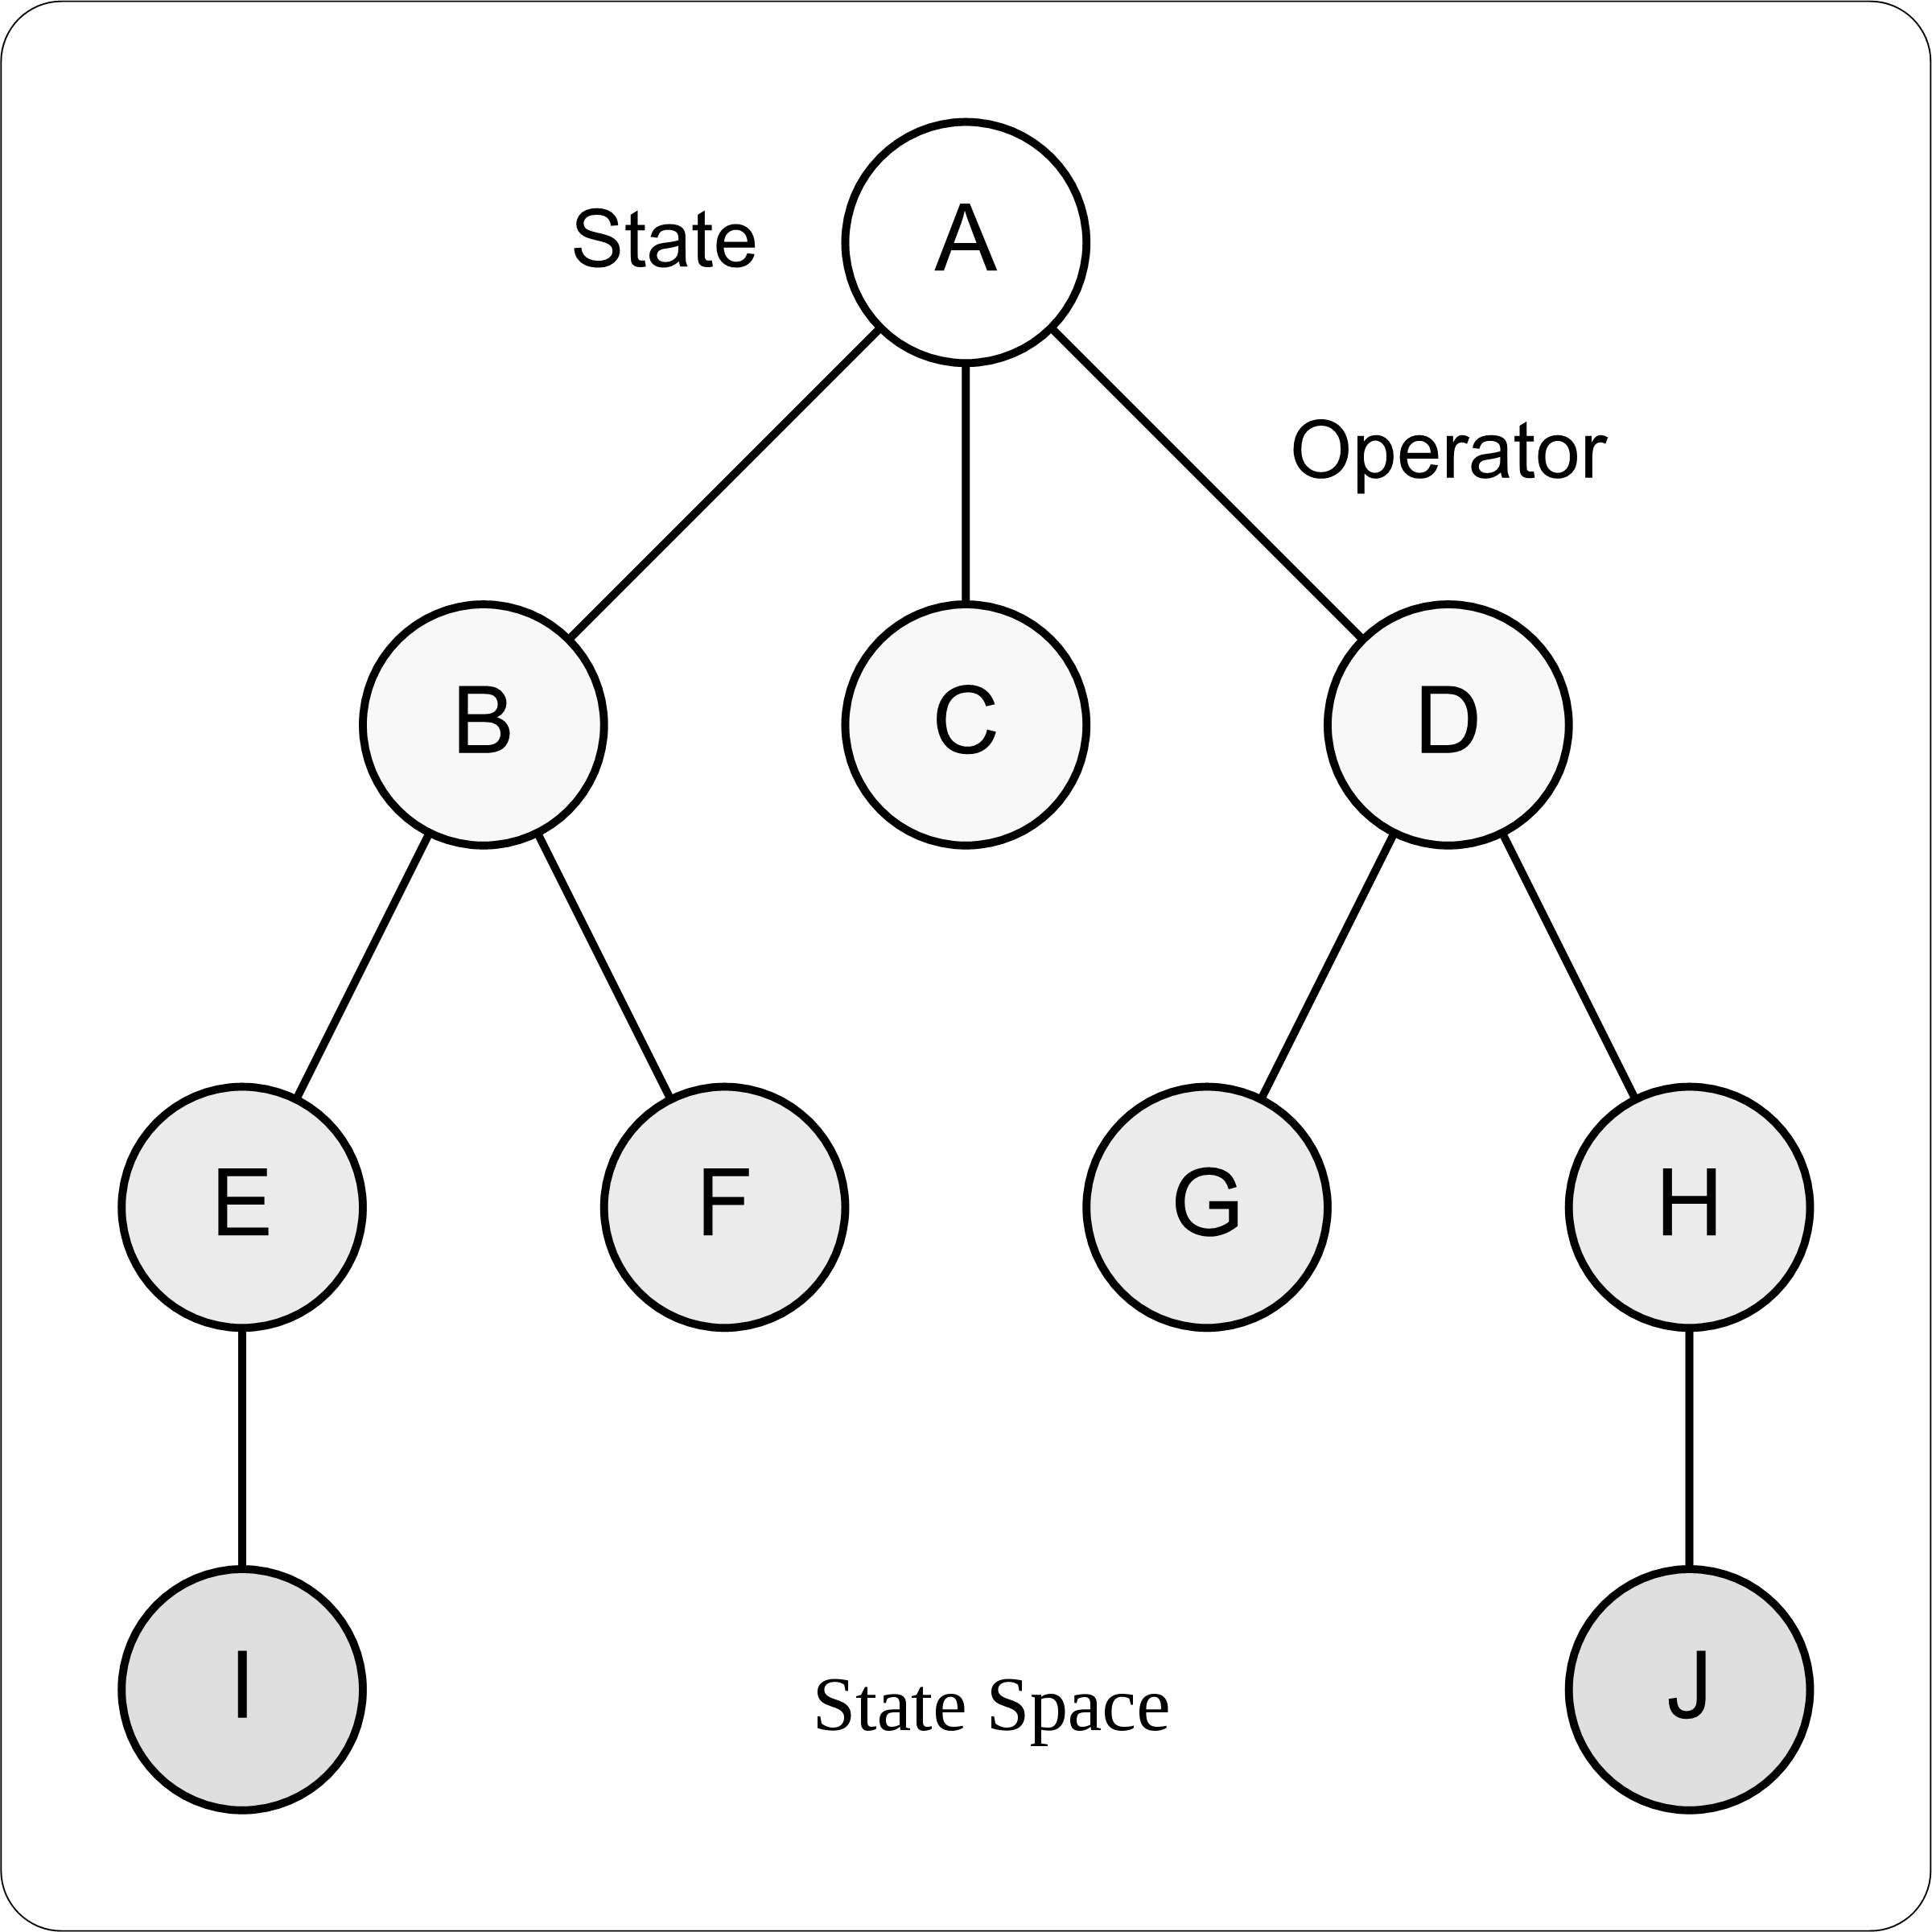
\includegraphics[width=.6\textwidth]{2c}
    \caption{Example of a state space represented with a graph. Courtesy of Bernt Arild Bremdal}
  \end{figure}
  \mysubsection{4}{D}
  Expression: $$P(\text{Rain}|\text{Dark Clouds})=\frac{P(\text{Rain}\cap\text{Dark Clouds})}{P(\text{Dark Clouds})}$$ Can be read as "Probability of rain given that we can observe dark clouds" or to generalize $$P(\text{A}|\text{B})$$ is a conditional probability of A occurring given that B is true.
  
  As such to calculate the probability I would need to first find out probability of rain which is $$\frac{\text{Rainy days}}{\text{All days}}$$ then I would need to calculate $$\frac{\text{Rainy days with dark clouds}}{\text{All days}}$$ and then divide latter by the former.
  \begin{figure}[H]
    \centering
    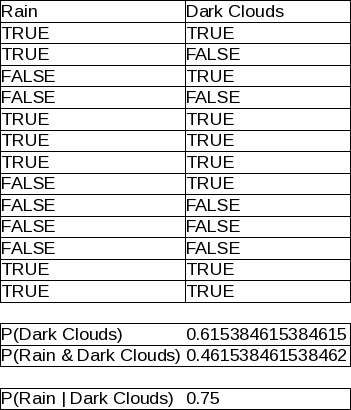
\includegraphics[width=.6\textwidth]{2d}
    \caption{Example of calculating $P(\text{Rain}|\text{Dark Clouds})$. OC do not steal}
  \end{figure}

  \mysubsection{5}{E}
  Backwards chaining is hypothesis driven, this means that we find facts that support at least one of hypothesis, it used most often with diagnostic.
  
  Forwards chaining on the other hand is a facts driven, this means that from a set of facts we create a conclusion.
  
  If we have same facts and conclusion then tree produced by backwards chaining will be the same as forwards chaining tree only turned upside down.
  \begin{figure}[H]
    \centering
    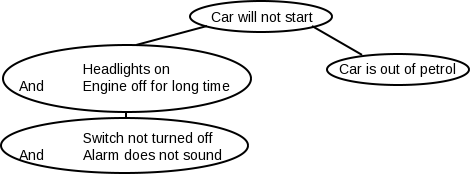
\includegraphics[width=.6\textwidth]{2e}
    \caption{Backwards chaining done on a set of facts where conclusion is that car will not start. OC do not steal}
  \end{figure}

  \mysubsection{6}{F}
  As we can see from the graph 19 is both member of Chilly and Warm groups, therefore we need to use the Sugeno defuzzyfication method. This is as follows
  \begin{align*}
    \text{Chilly} &= \underline{0.75}\\
    \text{Warm} &= \underline{0.35}\\
    \text{Energy for Chilly} &= 2000W \cdot 0.75 = \underline{1500W}\\
    \text{Energy for Warm} &= 200W \cdot 0.35 = \underline{70W}\\
    \text{Total energy output} &= \frac{1570}{1.1} = \uunderline{1427.\overline{27}W}\\
  \end{align*}
  
  \mysubsection{6}{G}
    \mysubsubsection{1}{1}
    By simply converting drawing to graph I get:
    \begin{figure}[H]
      \centering
      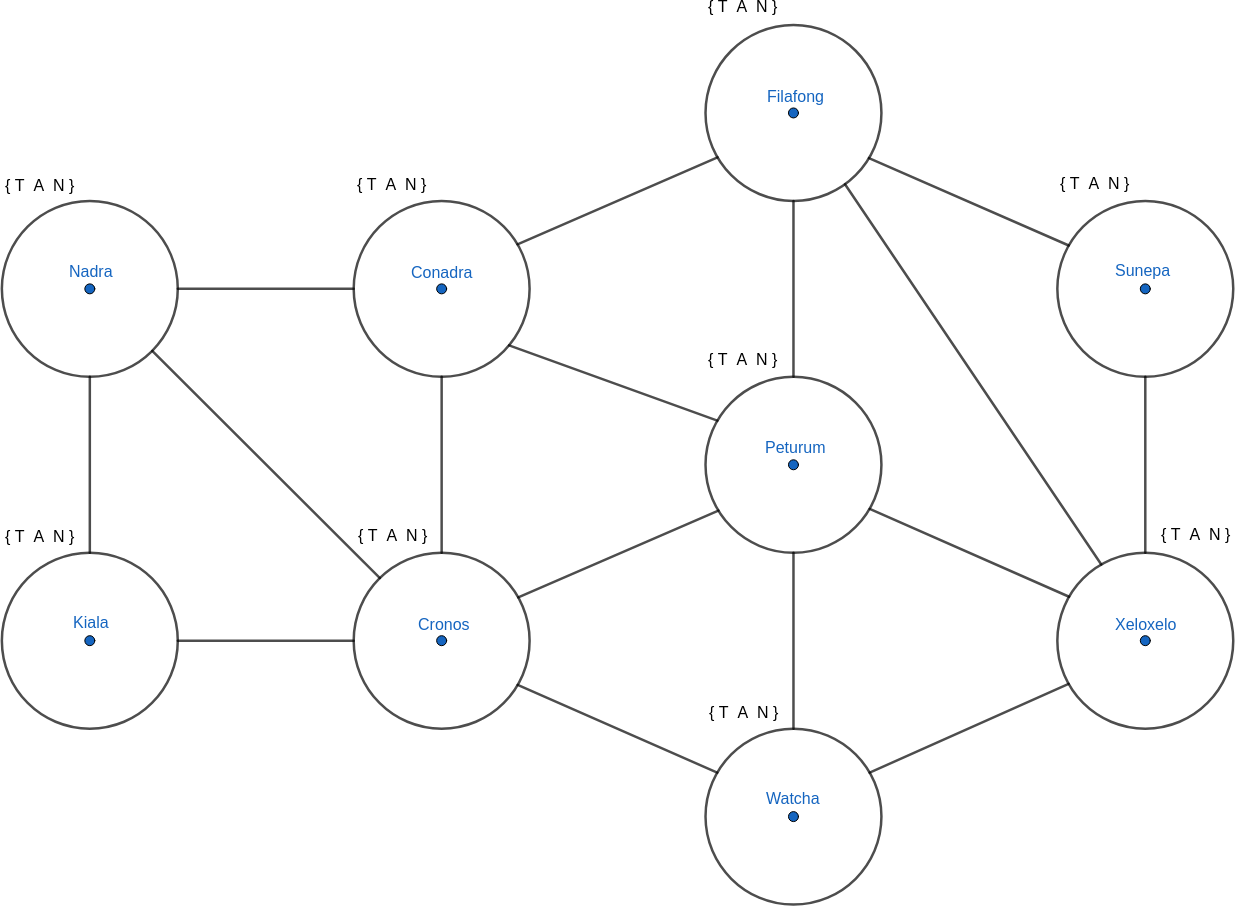
\includegraphics[width=.6\textwidth]{2g1}
      \caption{Constraint graph. OC do not steal}
    \end{figure}
   
    \mysubsubsection{2}{2}
    \begin{figure}[H]
      \centering
      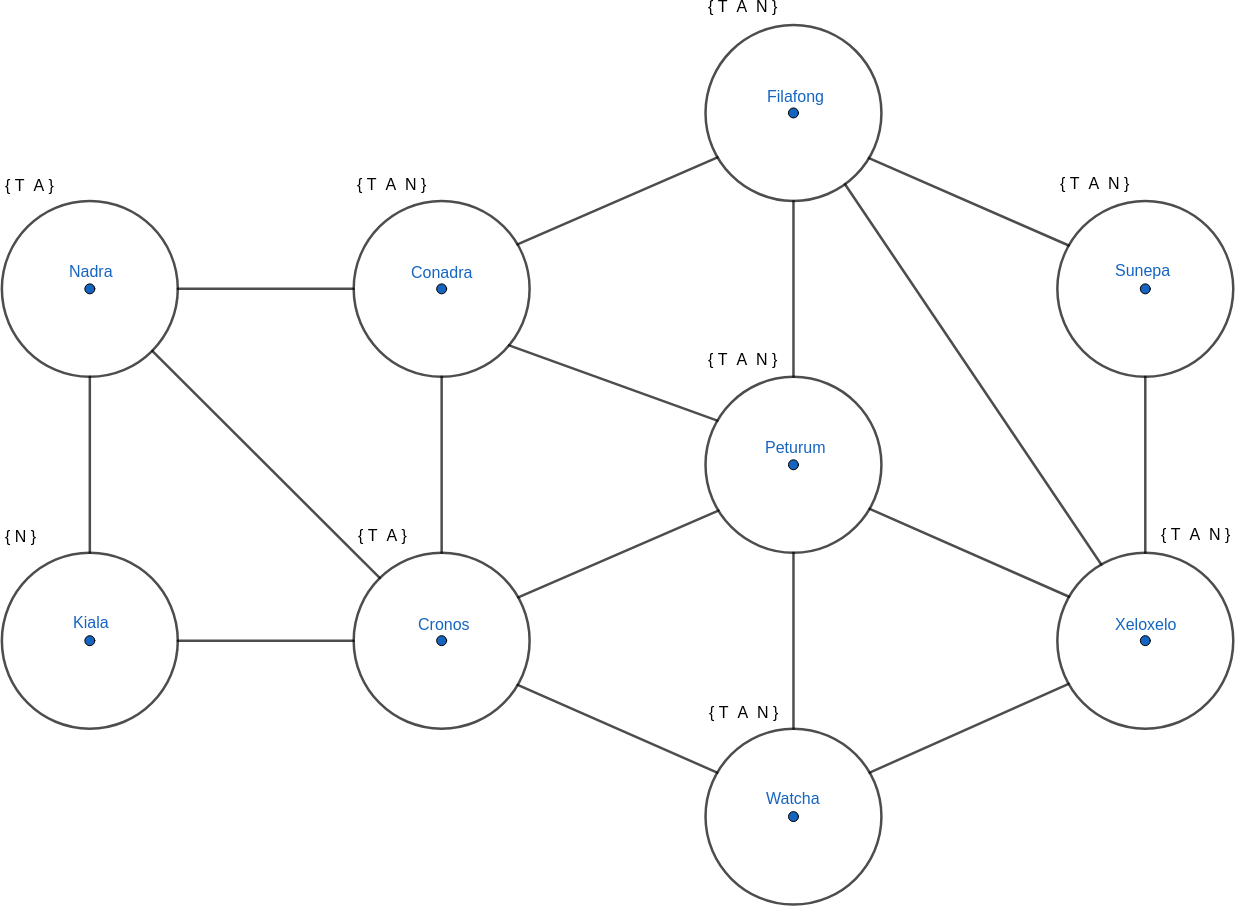
\includegraphics[width=.45\textwidth]{2g2}
      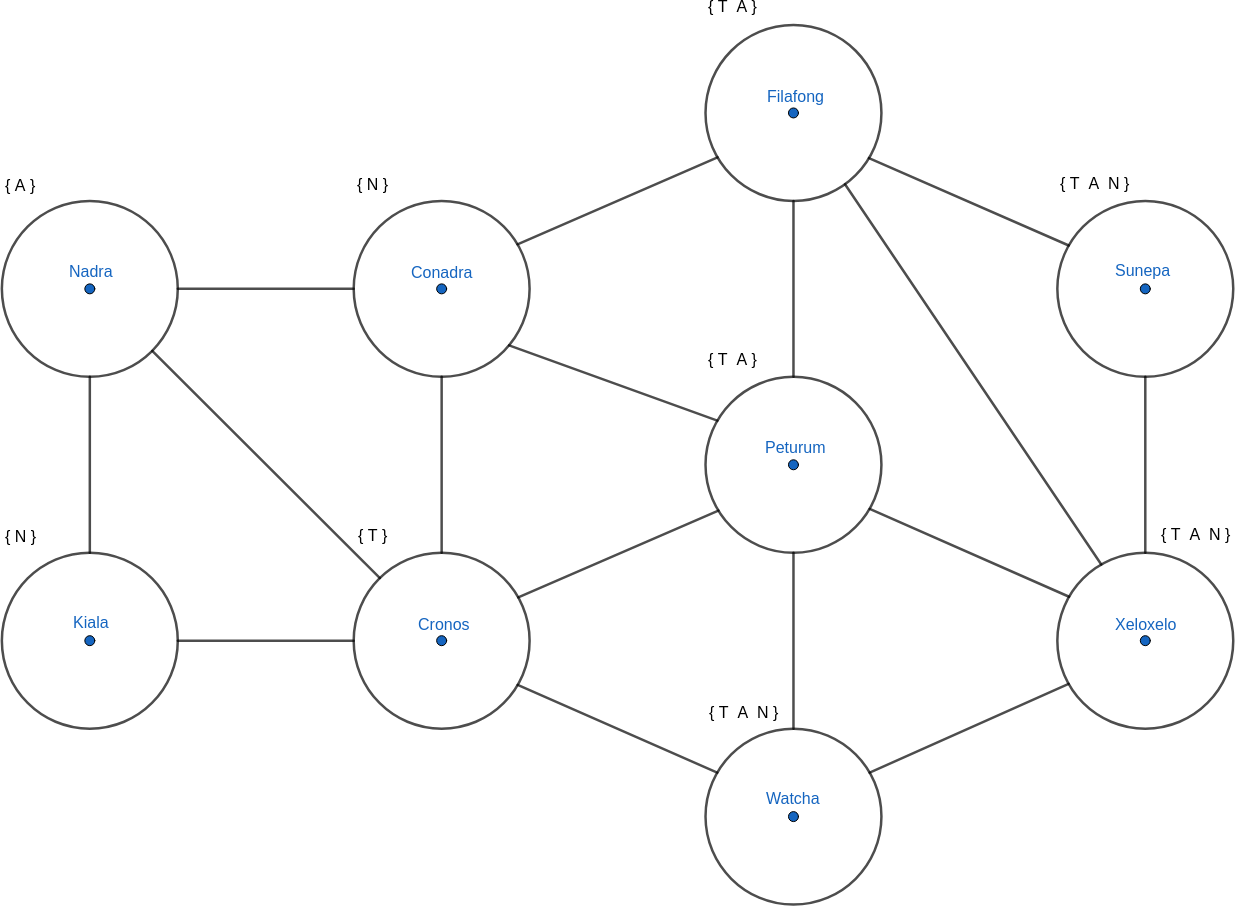
\includegraphics[width=.45\textwidth]{2g3}
      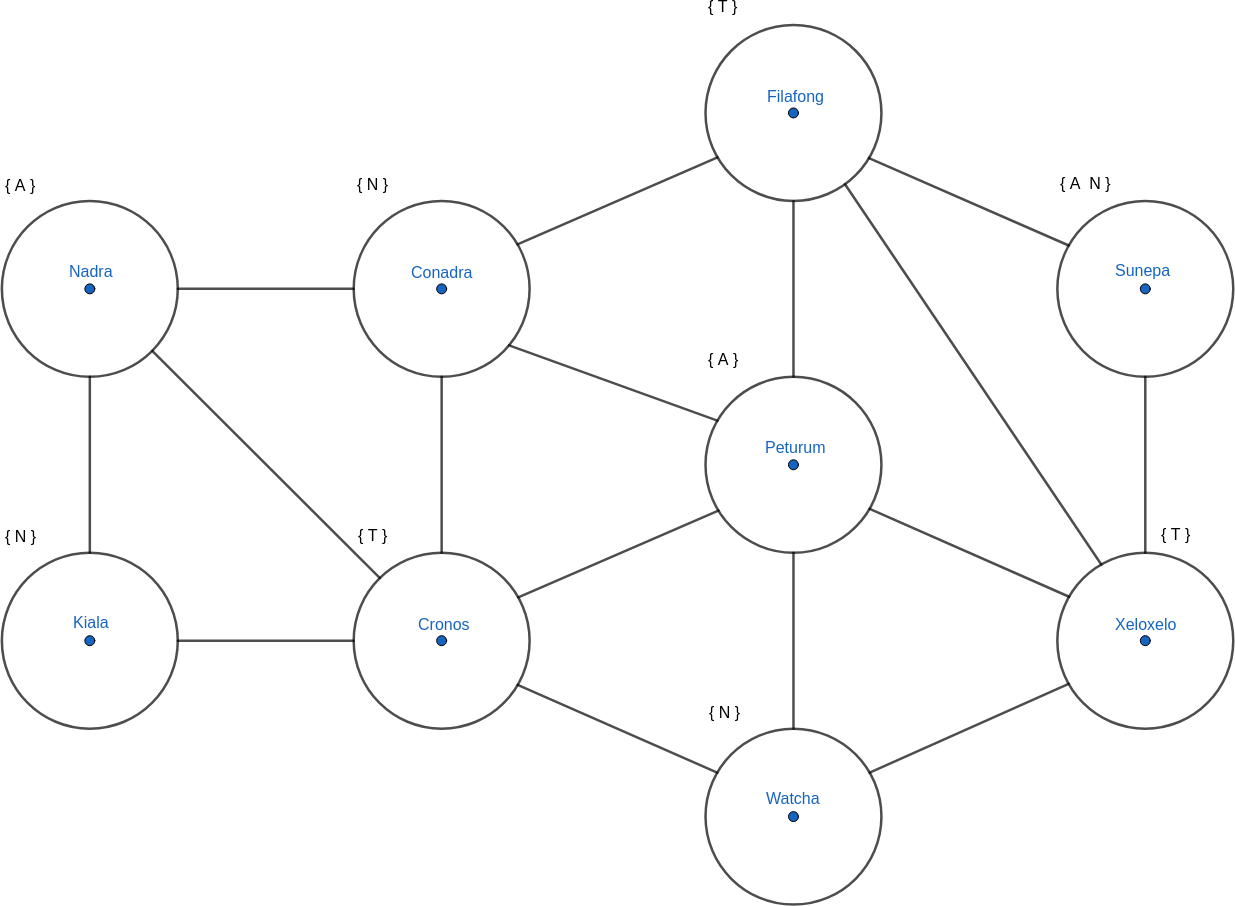
\includegraphics[width=.45\textwidth]{2g4}
      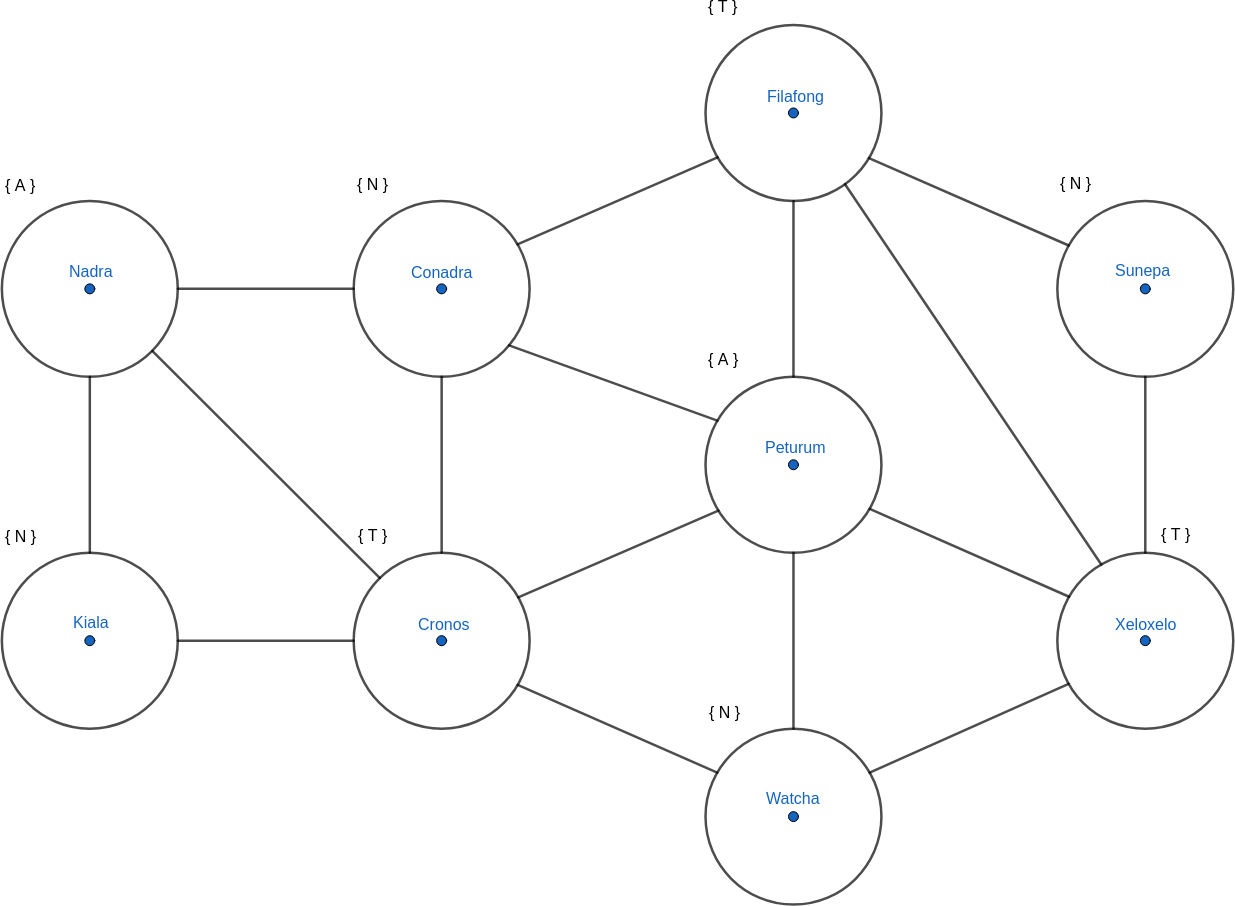
\includegraphics[width=.45\textwidth]{2g5}
      \caption{Progression of constraint propagation through graph}
    \end{figure}
    
    \mysubsubsection{3}{3}
    The division of Troops and Ambasadors after algorithm is:
    \begin{description}
      \item[Ambassador regions: ] Nadra, and Peturum.
      \item[Troop regions: ] Cronos, Filafong, and Xeloxelo.
      \item[None regions: ] Kiala, Conandra, Watcha, and Sunepa.
    \end{description}
  
    Algorithm cannot guarantee optimal solution as where we start and what option we choose can have an impact on the graph. In another run I end up with following distribution:
    \begin{description}
      \item[Ambassador regions: ] Cronos, and Filafong.
      \item[Troop regions: ] Kiala, Conandra, Watcha, and Xeloxelo.
      \item[None regions: ] Peturum, and Nadra.
    \end{description}
    
\end{document} 